% !TeX root = ../exam-zh-doc.tex

\section{安装与更新}


\subsection{标准安装}

目前 \cls{exam-zh} 已经上传 CTAN,您可以使用宏包管理器安装 \cls{exam-zh}。
例如在 \TeXLive{} 中,执行(可能需要管理员权限)
\begin{shellcode}[morekeywords={tlmgr,install}]
  tlmgr install exam-zh
\end{shellcode}
即可完成安装。

在 \TeXLive{} 和 \MiKTeX{} 中,您还可以通过图形界面进行安装,
此处不再赘述。


\subsection{手动安装}

您也可以通过访问 gitee 项目主页的方式获取最新版本的 \cls{exam-zh}(通常情况下,gitee 的版本会大于等于CTAN 的版本(因为 CTAN 从上传到审核到用户可以下载需要一天左右))。主要以「下载发行版」的方式获取最新版本的 \cls{exam-zh}:

\begin{enumerate}
  \item 进入项目主页(\href{https://gitee.com/zepinglee/exam-zh}{gitee 项目主页} (界面见图~\ref{figure:gitee项目主页} )
  \item 在右侧一列有“发行版”(gitee),并且有一个标签图标并有“vx.x.x - 20xx-xx-xx”字样,表示最新的发行版版本和发布时间,点击即可查看相关信息(如果想查看历史所有发行版信息,可以点击“发行版”右侧的“全部”(gitee))。
  
    发行版中一般由以下信息构成(\href{https://gitee.com/zepinglee/exam-zh/releases}{gitee 发行版} 界面见图~\ref{figure:gitee发行版})
      \begin{itemize}
        \item 更新文件的特别说明。如果没有,则表明此次更新只需要更新 \file{exam-zh.cls} 文件至最新\footnote{“更新 \meta{文件} 至最新”目前表示在发行版中下载最新版本的模板,并用其中所需要更新的 \meta{文件} 去替换本地的旧 \meta{文件}} 即可
        \item 更新日志。 主要为此次发行版与上次发行版的不同,一般为“Added”、“Changed”、“Fixed”等信息
        \item 模版及用户手册下载链接(“下载”部分)。一般用户只需要点击 \file{exam-zh-vx.x.x.zip} 进行模版下载即可,而下面的 \file{Source code} 为项目的整个源码,包括手册的源码,测试文件等,如果感兴趣的用户可以下载进行查看(当然,如果会使用 \cmd{git} 的用户也可以将整个 \cls{exam-zh} 项目 \cmd{clone} 下来查看)
      \end{itemize}
  \item 点击 \file{exam-zh-vx.x.x.zip} 进行下载,在本地解压即可
\end{enumerate}


\begin{figure}[htbp]
  \centering
  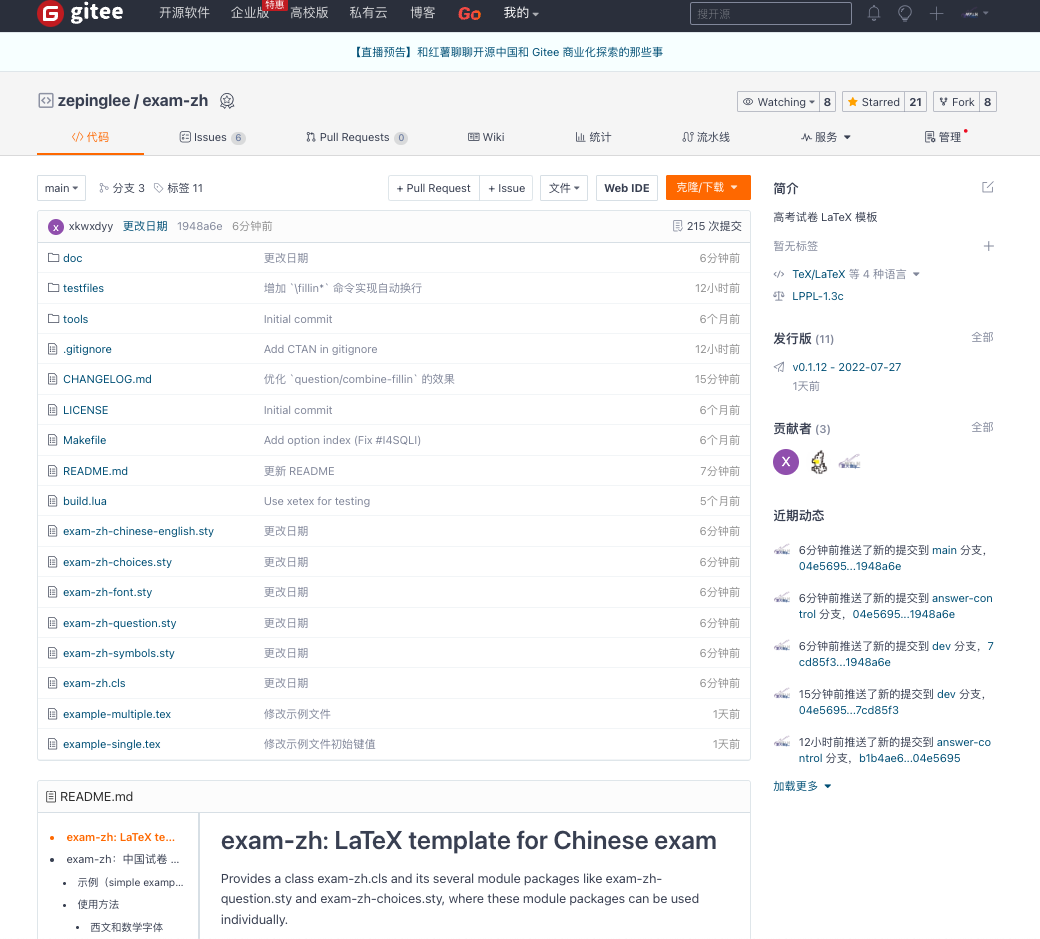
\includegraphics[width = \textwidth]{gitee-main.png}
  \caption{gitee 项目主页}
  \label{figure:gitee项目主页}
\end{figure}


\begin{figure}[htbp]
  \centering
  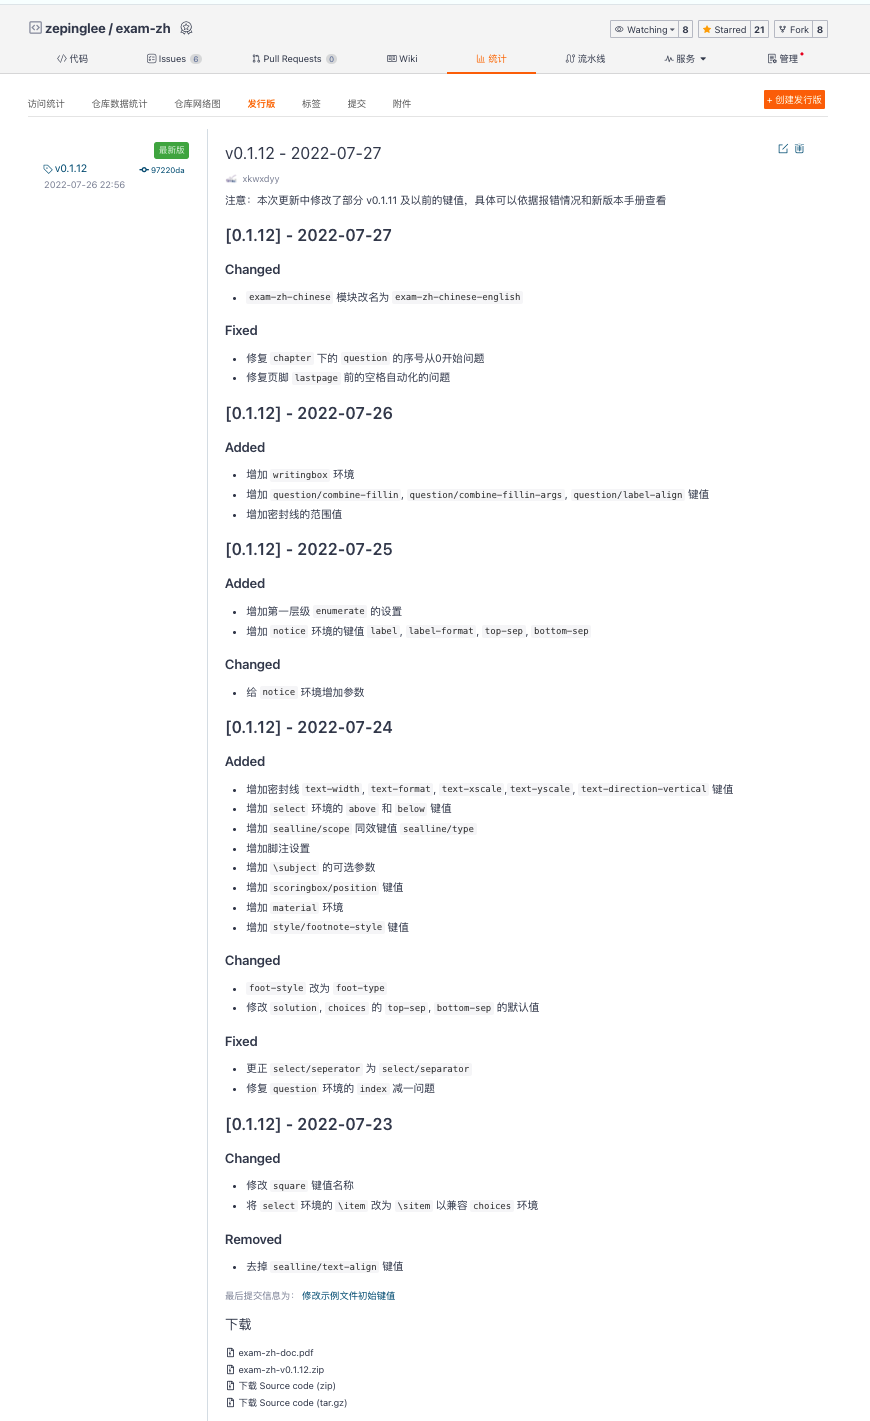
\includegraphics[width = 0.8\textwidth]{gitee-release.png}
  \caption{gitee 发行版}
  \label{figure:gitee发行版}
\end{figure}



\subsection{模板组成}

本模板主要包含核心文档类、参考文献格式文件以及用户文档等几个部分,
其具体组成见表~\ref{tab:exam-zh-main-components}。

\begin{table}[htbp]
  \caption{\cls{exam-zh} 的主要组成部分}
  \label{tab:exam-zh-main-components}
  \centering
  \small
  \begin{tblr}{
    hline{1, 2, Z} = {1pt},
    width = \textwidth,
    colspec = {X[3,l]X[5.5,l]},
    rows = {m}
  }
    \textbf{文件} & \textbf{功能说明} \\
    \file{exam-zh-doc.pdf}            & 用户手册(本文档) \\
    \file{example-single.tex}、\file{example-multiple.tex}            & 模板的主文件(同时也是示例文件),可据此为基础完成试卷编写 \\
    \file{exam-zh.cls}            & 模板文档类 \\
    \file{exam-zh-choices.sty}    & 模版的选择题模块宏包\\
    \file{exam-zh-question.sty}   & 模版的题干模块宏包\\
    \file{exam-zh-font.sty}       & 模版的字体模块宏包\\
    \file{exam-zh-symbols.sty}    & 模版的符号模块宏包\\
    \file{exam-zh-chinese-english.sty}    & 模版的语文英语模块宏包\\
    \file{README.md}              & 简要自述 \\
    \file{CHANGELOG.md}           & 模板更新日志 \\
    \file{LICENSE}                & 模版发布许可证
  \end{tblr}
\end{table}

% \begin{table}[htbp]
%   \caption{\cls{exam-zh} 各目录的组成部分}
%   \label{tab:exam-zh-sub-components}
%   \centering
%   \small
%   \begin{tblr}{
%     hline{4,5,8,11,13} = {solid},
%     hline{1, 2, Z} = {1pt},
%     width = \textwidth,
%     colspec = {X[1,l]X[3,l]X[3,l]},
%     rows = {m},
%     cell{2}{1} = {r=2}{m},
%     cell{5}{1} = {r=3}{m},
%     cell{8}{1} = {r=3}{m},
%     cell{11}{1} = {r=2}{m},
%   }
%     \textbf{子目录} & \textbf{子目录中的文件} & \textbf{功能说明} \\
%     front & \file{abstract.tex}            & 中英文摘要 \\
%     front & \file{notation.tex}            & 符号表 \\
%     body  & \file{chapter<number>.tex}     & 正文的分文件 \\
%     back  & \file{acknowledgements.tex}    & 致谢 \\
%     back  & \file{appendix.tex}            & 附录 \\
%     back  & \file{publications.tex}        & 攻读学位期间取得的研究成果(博士)\\
%     logo  & \file{ccnulogo.png}            & “华中师范大学”字样 logo \\
%     logo  & \file{masterlogo.png}          & 硕士学位论文页眉 logo \\
%     logo  & \file{doctorlogo.png}          & 博士学位论文页眉 logo \\
%     copyright  & \file{Originality_Copyright.pdf}  & 本科学位论文原创性声明和使用授权说明 \\
%     copyright  & \file{Originality_Copyright_master_doctor.pdf}  & 硕博学位论文原创性声明和使用授权说明\\
%     figures & & 用户放置图片的目录\\
%   \end{tblr}
% \end{table}